\section{Review}
\subsection{Convolutional Neural Nets Background}
In recent years, Convolutional Neural Nets (CNNs) have become more and more popular for image related tasks. First introduced by Yann Lecun, this particularly powerful neural network structure has become wide adopted by researches for their efficiency and robustness. Over the years, multiple papers attempts to improve performance of the CNN by changing activation functions or by augmenting the structure. However, most designs seem to share the same principle: they use alternating convolution and max-pooling layers followed by some number of fully connected layers. A typical convolution maxpooling sequence is shown in figure \ref{fig:cnn}. \\
\begin{figure}[hb]
	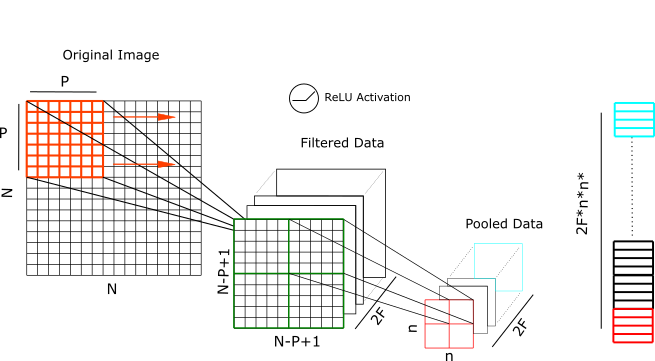
\includegraphics[width = 8cm]{img/CNN.png}
    \caption{\label{fig:cnn}
    An example architecture of a CNN.
    On the left is an 2D image input, followed by a convolutional layers, and a 
    max pooling layer. }
\end{figure}\\
The convolution layers defines a set of filters and an activation function. It convolve the input to that layer with its filters to generate an output which is then passed through the activation function. In this example, the convolution layer contains $2F$ filters of size $P\times P$; by convolving the $N\times N$ input with all of its filters, it generate $2F$ feature maps with size $(N-P+1)\times (N-P+1)$. The final output of the convolution layers are obtained by passing the feature maps through the ReLU function.
\begin{align}
	ReLU(x) = max(0,x)
\end{align}
The max-pooling layer down-scales the feature maps by dividing the feature maps into subsections and representing that entire subsection with the maximum value inside it.\\
Finally, at the end of the last max-pool layer, the feature maps are flattened into a vector which are usually used as the input to the fully connected layers are shown in Figure \ref{fig:fullyconnected}\\
In the fully connected layers, each node has a weighted connection to every node from the previous layer, it's output is determined by passing through the weighted sum of previous layer output through an activation function. The input is non-linear transformed through the layers and this non-linear transformation helps the neural net in finding separation between classes.\\
\begin{figure}[hb]
	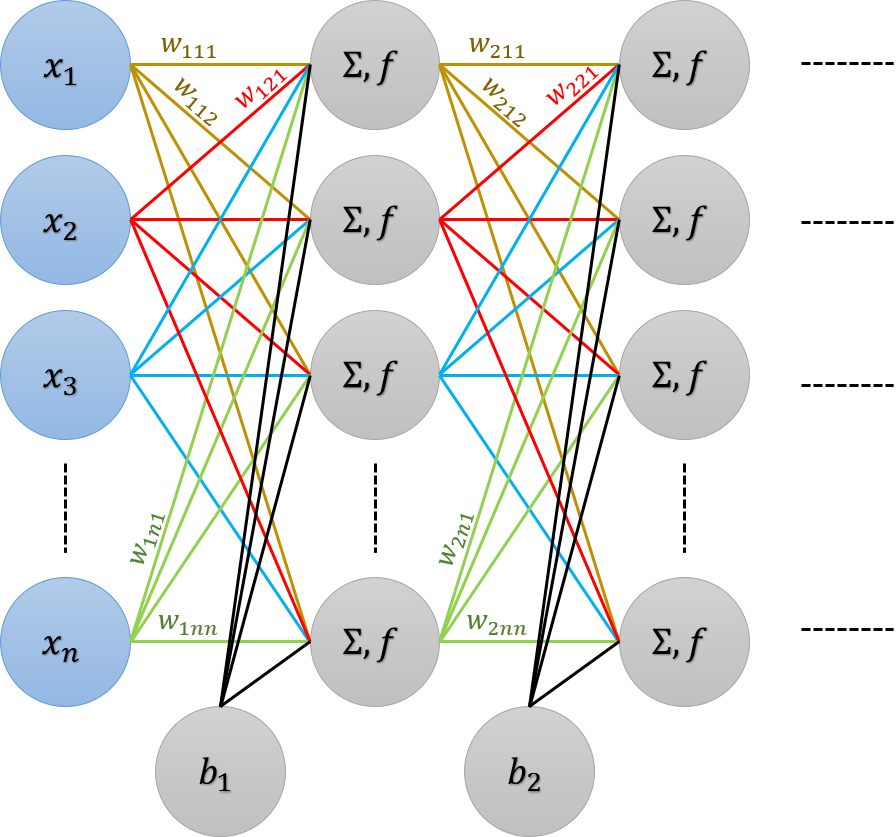
\includegraphics[width = 8cm]{img/fullyconnected.png}
    \caption{\label{fig:fullyconnected}
    Fully connected layers}
\end{figure}

\subsection{Homogeneous Structure}
The author challenges the conventional CNN structure by introducing a number of models that are increasing more homogeneous -- the most extreme of which contains only convolutional layers without pooling or fully connected layers.
According to the paper a pooling layer is equivalent to perform a feature-wise convolution by replacing the activation function with a $p$-norm. Thus, they question why a pooling layer is needed. Based on this questioning
they state the hypothesis that pooling is only important in order to reduce the dimensionality. Assuming this hypothesis is true, a pooling layer can be replaced by
a convolutional layer with an increased stride.

Additionally, by using convolutional layers with a filter size smaller than 5, the authors reduce the number of parameters in a network.
Moreover, they argument that fully connected layers are not necessary since units in the last convolutional layer in the network cover a sufficient portion of the image to be able to recognize it.
% Please proofread what I've written above
